\chapter{Koding Tingkat Medium}
Pada bagian ini akan dibahas berbagai pemrograman Python yang lebih {\em advanced}. Sebetulnya yang akan dibahas adalah contoh-contoh kode Python dengan menggunakan berbagai paket yang tersedia.

\section{Numpy}
Numpy adalah paket python untuk berbagai aplikasi {\em scientific}. Sebagai contoh, jika kita ingin membangkitkan bilangan random dengan distribusi tertentu (uniform atau normal), maka kita dapat menggunakan paket Numpy ini.

(Contoh-contoh penggunaan paket Numpy akan digabungkan dengan bagian lain.)

\section{Matlplotlib}
Salah satu aplikasi yang cukup sering dibutuhkan ketika kita membuat program untuk keperluan penelitian adalah membuat grafik (plot). Salah satu {\em library} yang baik untuk digunakan adalah {\em matplotlib}. Paket ini membutuhkan paket lain, yaitu {\em python-tk}. Untuk itu python-tk ini harus dipasang dulu. Di bawah ini adalah contoh pemasangan python-tk di sistem Linux (berbasis Debian) dengan menggunakan perintah apt-get.

\begin{verbatim}
$ sudo apt-get install python-tk
$ sudo pip install matplotlib
\end{verbatim}

Berikut ini adalah sebuah contoh penggunaan Matplotlib dan Numpy. Pada contoh ini kita akan membuat kumpulan data yang memiliki karakteristik ``sekitar'' persamaan 
$Y = Ax + b$.
Untuk itu perlu dihasilkan data yang sudah ditambahi atau dikurangi dengan angka random (yang dibuat dengan menggunakan Numpy). (Kode ini diambil dari buku ``Getting Started with Tensorflow''\cite{tensorflowstarted}.)
Hasilnya dapat dilihat pada gambar~\ref{fig:randomnumpy}


\begin{verbatim}
import numpy as np
import matplotlib.pyplot as plt

a = 0.25
b = 0.75
jumlah_titik = 300

# buat dua list yang masih kosong
x_point = []
y_point = []

for i in range(jumlah_titik):
    x = np.random.normal(0.0,0.4)
    y = a*x + b + np.random.normal(0.0,0.1)
    x_point.append([x])
    y_point.append([y])

plt.plot(x_point,y_point,'o',label='Random Data')
plt.legend()
plt.show()
\end{verbatim}


\begin{figure}[ht]
\fbox{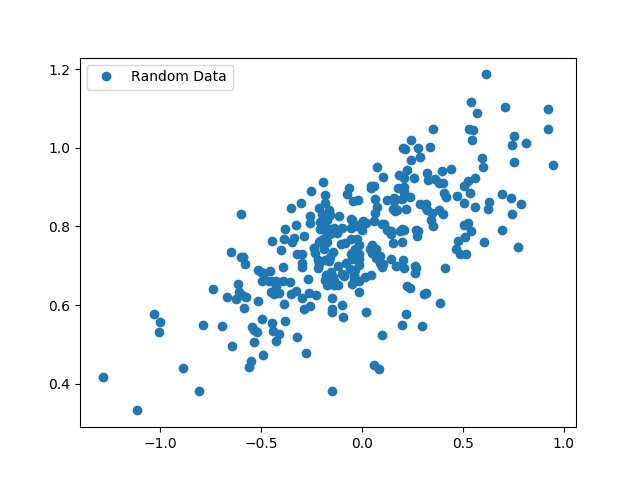
\includegraphics[width=1.0\linewidth]{graphics/random-data.png}}
\caption{Contoh Pembangkitan Random Data}
\label{fig:randomnumpy}
\end{figure}

\section{Pandas}
Pandas adalah library untuk data processing. Dia banyak digunakan untuk
berbagai aplikasi, seperti misalnya di Machine Learning.

Langkah pertama yang dilakukan adalah memasang Pandas.

\begin{verbatim}
$ sudo pip install pandas
\end{verbatim}


\section{Kriptografi}
Sebagaimana bidang lain, Python memiliki {\em library} yang lengkap untuk
kriptografi. Berikut ini hanya beberapa contoh penggunaan {\em library}
tersebut.

\subsection{Fungsi Hash}
Fungsi hash adalah fungsi satu arah yang memberikan tanda ({\em signature})
dari data digital; {\em stream of data} dan berkas.
Perubahan satu bit saja dari data tersebut akan mengubah nilai dari
{\em hash} yang dihasilkan. Itulah sebabnya fungsi {\em hash} dapat
digunakan untuk menjamin integritas data.

Ada banyak algoritma fungsi hash. Algoritma yang terkenal adalah MD5
dan SHA. Saat ini MD5 sudah dianggap tidak layak lagi karena sudah
ditemukan {\em collision}, yaitu nilai {\em hash} yang sama untuk data
yang berbeda. SHA~256 merupakan algoritma yang dianggap cocok saat ini.

\begin{verbatim}
unix$ echo "beli 10000" | shasum -a 256
375a6c46228994656932f4aa17d9ae50f21da75a31ff17f8517c255c06cba809 -

unix$ cat pesan1.txt
beli 10000
unix$ shasum -a 256 pesan1.txt
375a6c46228994656932f4aa17d9ae50f21da75a31ff17f8517c255c06cba809 pesan1.txt

unix$ cat pesan2.txt
beli 1000
unix$ shasum -a 256 pesan2.txt
5901bccc6a0556fac2b4a164ef831a7ed4ceddeb60c6ddde1162f5a40b9d2917 pesan2.txt
\end{verbatim}

Contoh kode Python untuk hal di atas adalah sebagai berikut:

\begin{verbatim}
# Contoh fungsi hash
import hashlib
h = hashlib.sha256("beli 10000\n")
print h.hexdigest()
\end{verbatim}


Salah satu pemanfaatan ``baru'' dari fungsi {\em hash} ini adalah pada
algoritma {\em Blockchain} yang digunakan pada {\em Bitcoin}. Sedikit
cerita tentang hal ini ada di blog
saya~\footnote{https://rahard.wordpress.com/2018/03/10/berburu-hash/}.
